\section{DTU-løb}

Løbet foregår i tværhold.

\subsection{Rotationsskema}

\begin{table}[H]
\centering
\begin{tabu}{l *{8}{L{1.4cm}}}\specialrule{1pt}{0pt}{2pt}
\rowfont{\bfseries}
Tid & Post 1 & Post 2 & Post 3 & Post 4 & Post 5 & Post 6 & Post 7 & Post 8 \\ \specialrule{1pt}{2pt}{2pt}
10:00 & 'Murica & Skotl & Ægypt & Ølymp & Buddh & Nord & Brasil & Austral \\ \specialrule{.25pt}{1pt}{1pt}
10:15 & Austral & 'Murica & Skotl & Ægypt & Ølymp & Buddh & Nord & Brasil \\ \specialrule{.25pt}{1pt}{1pt}
10:30 & Brasil & Austral & 'Murica & Skotl & Ægypt & Ølymp & Buddh & Nord \\ \specialrule{.25pt}{1pt}{1pt}
10:45 & Nord & Brasil & Austral & 'Murica & Skotl & Ægypt & Ølymp & Buddh \\ \specialrule{.25pt}{1pt}{1pt}
11:00 & Buddh & Nord & Brasil & Austral & 'Murica & Skotl & Ægypt & Ølymp \\ \specialrule{.25pt}{1pt}{1pt}
11:15 & Ølymp & Buddh & Nord & Brasil & Austral & 'Murica & Skotl & Ægypt \\ \specialrule{.25pt}{1pt}{1pt}
11:30 & Ægypt & Ølymp & Buddh & Nord & Brasil & Austral & 'Murica & Skotl \\ \specialrule{.25pt}{1pt}{1pt}
11:45 & Skotl & Ægypt & Ølymp & Buddh & Nord & Brasil & Austral & 'Murica \\ \specialrule{1pt}{2pt}{0pt}
\end{tabu}
\end{table}

\subsection{Poster og lokationer}

\begin{enumerate}
 \item Polyteknisk Forening - Struktur, faglige råd og udvalg - \textit{Gårdsplads} - \clint
 \item Kollegier - PKS og udlandsophold - \textit{Gang ved siden af "Kongressen"} - \karla
 \item PF Skitur - \textit{Græsplæne foran køkken} - \buddha
 \item S-Huset, Fredagsbarer og Joints - \textit{Større græsplæne til venstre for køkken} - \hemorides
 \item AUS/Studievejledningen - \textit{Rusværelse (Uddeles på turen)} - \mighty
 \item Puma-dansen - \textit{Spisesalen} - \randildo
 \item Tip en vektor - \textit{Pejsestuen} - \farav
 \item Noget, som sandsynligvis er dumt - \textit{Sal foran køkken} - \Hyttebums{Hyttebumz'erne}
\end{enumerate}


%%%%%%%%%%%%%%%%%%%%% Post 1 %%%%%%%%%%%%%%%%%%%%%
\subsubsection*{\textbf{Post 1 - Polyteknisk Forening - Struktur, faglige råd og udvalg}}
\subsubsection*{\textbf{Ansvarlig:} \Clint}

Hvor mange har allerede meldt sig ind i PF? \Hashtag{GodBeslutning}

\begin{itemize}
 \item En forening af de studerende, for de studerende.
 \item En 3-dimensionel forening, der engagerer sig både Fagligt, Politisk, Socialt og på alle områder imellem.
\end{itemize}

\begin{figure}[H]
\centering
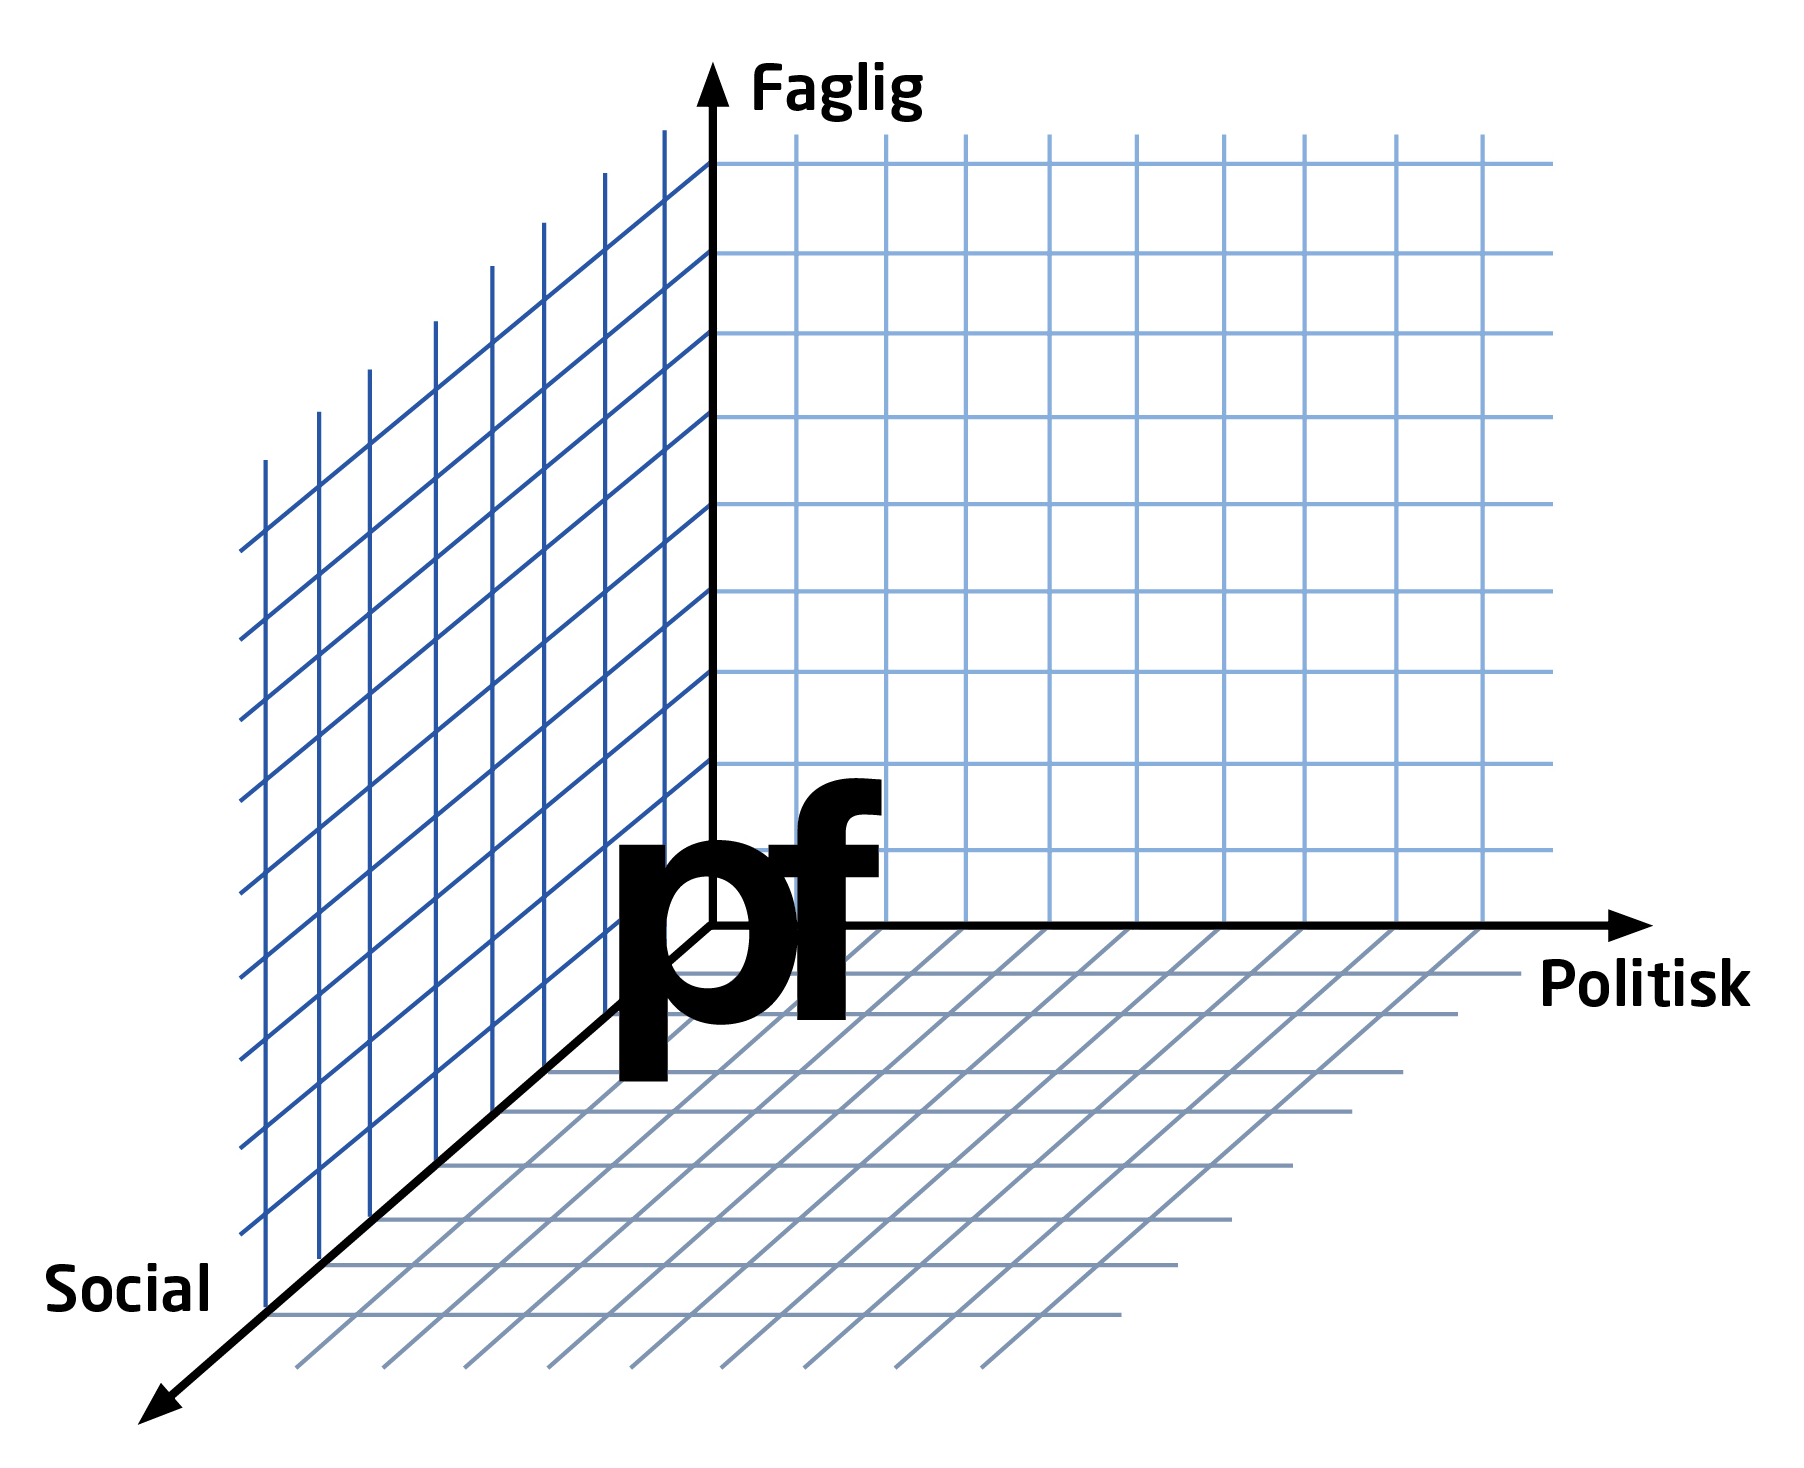
\includegraphics[width=\linewidth]{fig/PF.png}
\end{figure}

\begin{itemize}
 \item Fagligt
 \begin{itemize}
  \item Institutstudienævn - Evaluerer kurser og undervisere, for at sikre en høj kvalitet af undervisningen.
 \end{itemize}
 \item Politisk
 \begin{itemize}
  \item Uddannelsespolitisk råd - Sidder med i blandt andet DTU's bestyrelse, og deltager i diskussioner om uddannelsespolitik, der vedrører studerende på DTU.
 \end{itemize}
 \item Socialt
 \begin{itemize}
  \item S-Huset - Mere information hos \hemorides.
  \item Idræt og klubber - Fodbold, Badminton, Basket, Volley, Løb, Bordtennis, Dans, Klatring, Sejlads, Ølbowling, Brætspil, Foto, Poker etc. Få støtte til at oprette en ny PF klub (PF Camping?). I kommer til at møde klubberne på en rundvisning i semsteruge 3.
 \end{itemize}
 \item Rabatter
 \begin{itemize}
  \item Ulykkesforsikring, Fitness World, Lyngby Svømmehal, Briller, Aviser og meget mere...
 \end{itemize}
\end{itemize}

Aktiv i de faglige råd.

Indmelding: www.pf.dk

Spørgsmål?

Alle hold sendes videre til Kollegier og PKS på gangen ved siden af "Kongressen" hos \Karla


%%%%%%%%%%%%%%%%%%%%% Post 2 %%%%%%%%%%%%%%%%%%%%%
\subsubsection*{\textbf{Post 2 - Kollegier, PKS og udlandsophold}}
\subsubsection*{\textbf{Ansvarlig:} \Karla}

Indstilling til kollegierne sker gennem Polyteknisk Forenings IndstillingsUdvalg (PFIU). Ansøgning sker gennem www.pks.nu. Fortæl lidt om de forskellige kollegier og deres barer.
\begin{itemize}
 \item Kampsaxkollegiet - Saxen (Torsdag)
 \item Andelskollegiet - placering
 \item Prof. Ostenfeldt - Nakkeosten (1. tirsdag i måneden)
 \item Willum Kann Rasmussen - VKR-Baren (Mandag, ej lovlig)
 \item William Demant - Willys vandhul (Onsdag)
 \item P.O. Pedersen - Falladen (Tirsdag og lørdag)
 \item Paul Bergsøe - Pauls Ølstue (Tirsdag og fredag)
 \item Trørød (Par og unge med børn)
 \item Nybrogård - Kældercafeen (Fredag + evt. temafest om lørdagen) - Søges gennem KAB og ikke PKS
 \item Viggo Jarls -  - Søges gennem ?
\end{itemize}
Det meste information kan findes i rusbogen. Priser fra 2250-3300 kr.

\textbf{Udlandsophold:}\\
Rigtig mange vælger at tage et semester eller to i udlandet. Det er fedt.
\begin{itemize}
\item Skal søges et halvt til et helt år før afhængig af destination
\item DTU har aftaler med en række universiteter og sørger for SU, bolig og indskrivning hos disse
\item Søger man andre universiteter kan det gøres hos EF eller andre organisationer, så skal man selv klare ovenstående
\item Der er rigtig mange legater man kan søge - også selvom man får SU
\item Man kan få hjælp hos International Affairs i administrationen i 101
\item Praktikophold kan søges hos IAESTE (International Association for the Exchange of Students for Technical Experience)
\end{itemize}


Alle hold sendes videre til PF Skitur på plænen foran køkkenet hos \Buddha


%%%%%%%%%%%%%%%%%%%%% Post 3 %%%%%%%%%%%%%%%%%%%%%
\subsubsection*{\textbf{Post 3 - PF Skitur}}
\subsubsection*{\textbf{Ansvarlig:} \Buddha}
Uge 5 - 30. januar-8. februar
Sestriere, Italien
3295,- for ophold, bus tur/retur, Fester før og under mm. 
Buddha winger den.

Alle hold sendes videre til S-Huset og fredagsbarer på plænen til venstre for køkkenet hos \Hemorides

%%%%%%%%%%%%%%%%%%%%% Post 4 %%%%%%%%%%%%%%%%%%%%%
\subsubsection*{\textbf{Post 4 - S-Huset, fredagsbarer og joints}}
\subsubsection*{\textbf{Ansvarlig:} \Hemorides}
S-huset er placeret i bygning 101 og åbner alle hverdag kl. 7.30 og lukker igen når festen i Kælderbaren er gået kold (dog senest kl. 5.00).

\textbf{Kaffestuen:} mad og drikke. Special pris på bl.a. kaffe til PF medlemmer. Åben: Man-Fre: 07:30–19:00\\
\textbf{Pejsestuen:} Hyggeområde; sofaer, poolbord og bordfodboldbord.\\
\textbf{Læsesalen:} Bagerste lokale i S-huset. Brug biblio i stedet? God til eksamensforberedelse.\\
\textbf{Kælderbaren:} Specialøl, nyrenoveret, \Hashtag{Awesomeness} Åben: 19:00-?? (senest 05:00)\\

\textbf{PF Caféen:} S-huset består også af PF-Caféen i bygning 306. Lige overfor der hvor I har Mat 1. Åben: Man-Fre: 07:30 – 17:00\\


\textbf{Fredagsbarer}: Åbningstider 12:00-21:00 (eller 12:00-03:00 ved lang åbning). Hegnet åbner først 14:00 pga. Kantinen.
\begin{itemize}
  \item Diagonalen - Bygn. 116
  \item Etherrummet - Bygn. 208
  \item Hegnet - Bygn. 342
  \item Maskinen - Bygn. 358
  \item Diamanten - Bygn. 414
\end{itemize}

\textbf{Joints:}
\begin{itemize}
  \item Sensommerfest - 5. september
  \item Rusjoint - 12. september (Spiser sammen i tværgrupper - billetter ryger hurtigt)
  \item Oktoberfest - 2-3. oktober
  \item (PF-fest - 9. oktober) - MÅSKE!!!
  \item Seriøst motionsløb - 9. oktober
  \item Useriøst motionsløb - 10. oktober
  \item Julejoint - ??
\end{itemize}

Alle hold sendes videre til AUS og Studievejledningen på Rusværelset hos \Mighty


%%%%%%%%%%%%%%%%%%%%% Post 5 %%%%%%%%%%%%%%%%%%%%%
\subsubsection*{\textbf{Post 5 - AUS, Studievejledningen og den nye reform}}
\subsubsection*{\textbf{Ansvarlig:} \Mighty}
Afdelingen for Uddannelse og Studerende befinder sig i 101A. Alle spørgsmål om SU, dispensationer og andet kan stilles her. Desuden kan studievejledningen hjælpe med tekniske detaljer om merit, studieforløb, retningsskifte, og meget andet.
KKO, Studenterrådgivningen og Studiepræsten.

\subsection*{Studiefremdriftsreformen}
Ansvarlig: \Mighty
Til oplæg om AUS. 
\subsubsection*{Fag og prøver}
\label{sub:fag_og_pr_ver}
\begin{itemize}
  \item{Tilmelding til fag} Alle studerende \emph{skal} være tilmeldt kurser svarende til 30 \emph{nye(!)} ECTS-point hvert halvår (13-ugers + 3-ugers).
  \item{Tilmelding til prøver} ALLE studerende tilmeldes automatisk eksaminer i de fag, de er tilmeldt. Så snart eftertilmeldingsperioden er slut, kan man ikke vælge fag om, og er i udgangspunktet forpligtet til at bestå eksamen. Hvis man dumper, skal man til reeksamen næste semester eller i en særlig reeksamensperiode.
  \item{Studiestartsprøve} Inden for de to første måneder afholdes en prøve som \emph{skal} bestås for at kunne fortsætte på sit studie.
\end{itemize}

\subsubsection*{SU}
\label{sub:SU}
\begin{itemize}
  \item{Støttetidsregler} Hvis man søger ind på en videregående uddannelse for første gang senest to år efter endt gymnasiel uddannelse, har man 12 SU-klip ud over normeret studietid. Hvis man starter mere end to år efter endt gymnasielt stuie, er man kun berettiget til SU på normeret studietid.
  \item{SU-stop} Hidtil har man kunnet være 12 måneder bagefter med studiet, før SU'en inddrages. Disse regler ændres til 6 måneder, men træder først i kraft pr. \emph{1. september 2016}.
\end{itemize}


Alle hold sendes videre til Puma-dansen i Spisesalen hos \Randildo


%%%%%%%%%%%%%%%%%%%%% Post 6 %%%%%%%%%%%%%%%%%%%%%
\subsubsection*{\textbf{Post 6 - Puma-dansen}}
\subsubsection*{\textbf{Ansvarlig:} \Randildo}
Dans for helvede! DAAAAAAANS!!! (Reklamer for Rusjoint). \\
Alle hold sendes videre til Tip en Vektor i Pejsestuen hos \Farav


%%%%%%%%%%%%%%%%%%%%% Post 7 %%%%%%%%%%%%%%%%%%%%%
\subsubsection*{\textbf{Post 7 - Tip en Vektor}}
\subsubsection*{\textbf{Ansvarlig:} \Farav}
Hvad mon der skal foregå her?\\
Alle hold sendes videre til \Hashtag{NogetDumtOgFarligt} i salen foran Køkkenet hos \Hyttebums{De stive sørøvere}


\subsubsection*{\textbf{Post 8 - [Indsæt dum og farlig titel]}}
\subsubsection*{\textbf{Ansvarlig:} \Hyttebums{Piraterne}}

\Hashtag{NogetDumtOgFarligt}

Alle hold sendes videre til PF struktur i Gårdspladsen hos \Clint